    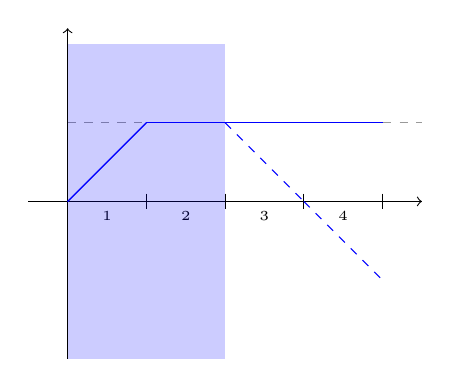
\begin{tikzpicture}
        % Draw x-axis

        \draw[->] (-.5,0) -- (4.5,0);
        \draw[dashed, opacity=0.4] (0,1) -- (4.5,1);
        % Draw y-axis
        \draw[->] (0,-2) -- (0,2.2);


        % Add ticks on x-axis
        \foreach \x in {1,2,3,4}
            \draw (\x,0.1) -- (\x,-0.1);
        
        \foreach \x in {1,2,3,4}
            \draw (\x - 0.5 ,0) -- (\x-0.5,-0)  node[below, font=\tiny] {\x};

        % Shade a vertical region
        \foreach \x in {1, 2}
            \fill[blue, opacity=0.2] (\x-1,-2) rectangle (\x,2);
        \draw[-, blue] (0, 0) -- (1, 1);\draw[-, blue] (1, 1) -- (2, 1);\draw[-, blue] (2, 1) -- (3, 1);\draw[-, blue] (3, 1) -- (4, 1);
        
        \draw[blue, -] (0, 0) -- (1, 1);\draw[blue, -] (1, 1) -- (2, 1);\draw[blue, dashed] (2, 1) -- (3, 0);\draw[blue, dashed] (3, 0) -- (4, -1);
            
    \end{tikzpicture}

    